\section{Gravitational-Wave signals from binary neutron star mergers}
\textcolor{blue}{Explain the use for this section.}\\
Gravitational waves from two inspiraling neutron stars are among the most interesting signals gravitational wave detectors can detect. They convey information about the highly relativistic regimes of gravity, about the structure of the component stars and about the formation channels of black holes or heavy neutron stars. \textcolor{red}{[Citations]} They are however also very hard to detect, as binary neutron star (\gls{bns}) systems are very light systems, when compared to inspiraling binary black holes (\gls{bbh}).\\
Part 1 of this section will discuss how gravitational waves (\gls{gw}) are formed and what influences the structure of the resulting waveforms. Part 2 will go over the current method of detecting \gls{gw} and discuss the advantages and drawbacks. \textcolor{red}{Need to specify, that I use Einstein sum convention in this section and that latin indices are spacial indices, whereas greek indices are over all four components. NEED TO CHANGE MOST CITATIONS FROM BACHELOR THESIS TO ORIGINAL SOURCES! Mention bachelor thesis only as a way to look up detailed calculations.}
\subsection{The waveform}
\textcolor{blue}{Explain how the waveform looks like, what it depends on, maybe give the concept how it works in the context of linearized theory (quote bachelor thesis), cite important papers regarding the waveform theory.}\\
Gravitational waves are a solution to the Einstein-equation
\begin{equation}\label{def:einstein_equation}
\mathcal{G}_\mn = \frac{8\pi G}{c^4}T_\mn,
\end{equation}
where $\mathcal{G}_\mn$ is the Einstein-tensor, $T_\mn$ is the energy-momentum-tensor, $G$ is the gravitational constant and $c$ is the speed of light in vacuum. They can be derived in their linear form, by setting assuming the metric to be a linear correction to the flat metric $\eta_\mn$
\begin{equation}\label{def:linear_approximation}
g_\mn = \eta_\mn + h_\mn.
\end{equation}
With this approximation the Einstein-equation \eqref{def:einstein_equation} simplifies to
\begin{equation}\label{def:einstein_linear}
\mathcal{G}_\mn=\frac{1}{2}\lr{\partial_{\alpha\mu}h^\alpha_\nu+\partial^\alpha_\nu h_{\mu\alpha} - \partial_\mn h- \Box h_\mn - \eta_\mn\Box h} = \frac{8\pi G}{c^4}T_\mn,
\end{equation}
where $h\coloneqq\eta^\mn h_\mn$ and $\Box\coloneqq\eta^\mn\partial_\mn$.\\
This equation has $10$ independent components, of which only $2$ are physical. To reduce the number of independent components, one can choose gauge conditions through the coordinate transformation ${x'}^\mu=x^\mu+\xi^\mu$, which leaves the Einstein equation invariant. One of these gauge conditions is the DeDonder gauge
\begin{equation}
\partial^\alpha \bar{h}_{\alpha\mu} = 0,
\end{equation}
where $\bar{h}_\mn\coloneqq h_\mn - \frac{1}{2}\eta_\mn h$. It can be realized by choosing $\Box\xi_\mu =\partial^\alpha \bar{h}_{\alpha\mu}$. In this gauge the linearized Einstein equation \eqref{def:einstein_linear} reduces to
\begin{equation}\label{def:gw_equation}
\Box\bar{h}_\mn=-\frac{16\pi G}{c^4}T_\mn.
\end{equation}
This gauge however leaves another freedom, as another transformation ${x'}^\mu=x^\mu+\xi^\mu$ could be applied, when $\Box\xi_\mu =0$. This can be used, such that the gauge to also satisfy $\bar{h}=-h=0$ and $\bar{h}_{0\mu} = 0 = \bar{h}_{3\mu}$. The gauge is named transverse-traceless-gauge (\gls{tt}) and results in the metric to be of the form
\begin{equation}\label{def:tt_gauge}
h_\mn^\text{\gls{tt}}=
\begin{pmatrix}
	0 & 0         & 0        & 0\\
	0 & h_+       & h_\times & 0\\
	0 & -h_\times & h_+      & 0\\
	0 & 0         & 0        & 0\\
\end{pmatrix}.
\end{equation}
\eqref{def:tt_gauge} now has only the two independent components $h_+$ and $h_\times$ left, which are called the ''plus-'' and ''cross-polarization'' of a \gls{gw}.\medskip\\
Evaluating \eqref{def:gw_equation} in vacuum reveals the wave-like character of $h_\mn$, as
\begin{equation}\label{def:gw_wave_equation}
\Box\bar{h}_\mn =0
\end{equation}
is a wave equation. Its solutions travel at the speed of light. Therefore \gls{gw} travel through space-time at the speed of light. The effect a solution of this equation has on a ring of resting test masses is shown in \autoref{fig:gw_test_masses}. (chapter 3 \cite{bachelor})\medskip\\
\begin{figure}
\centering
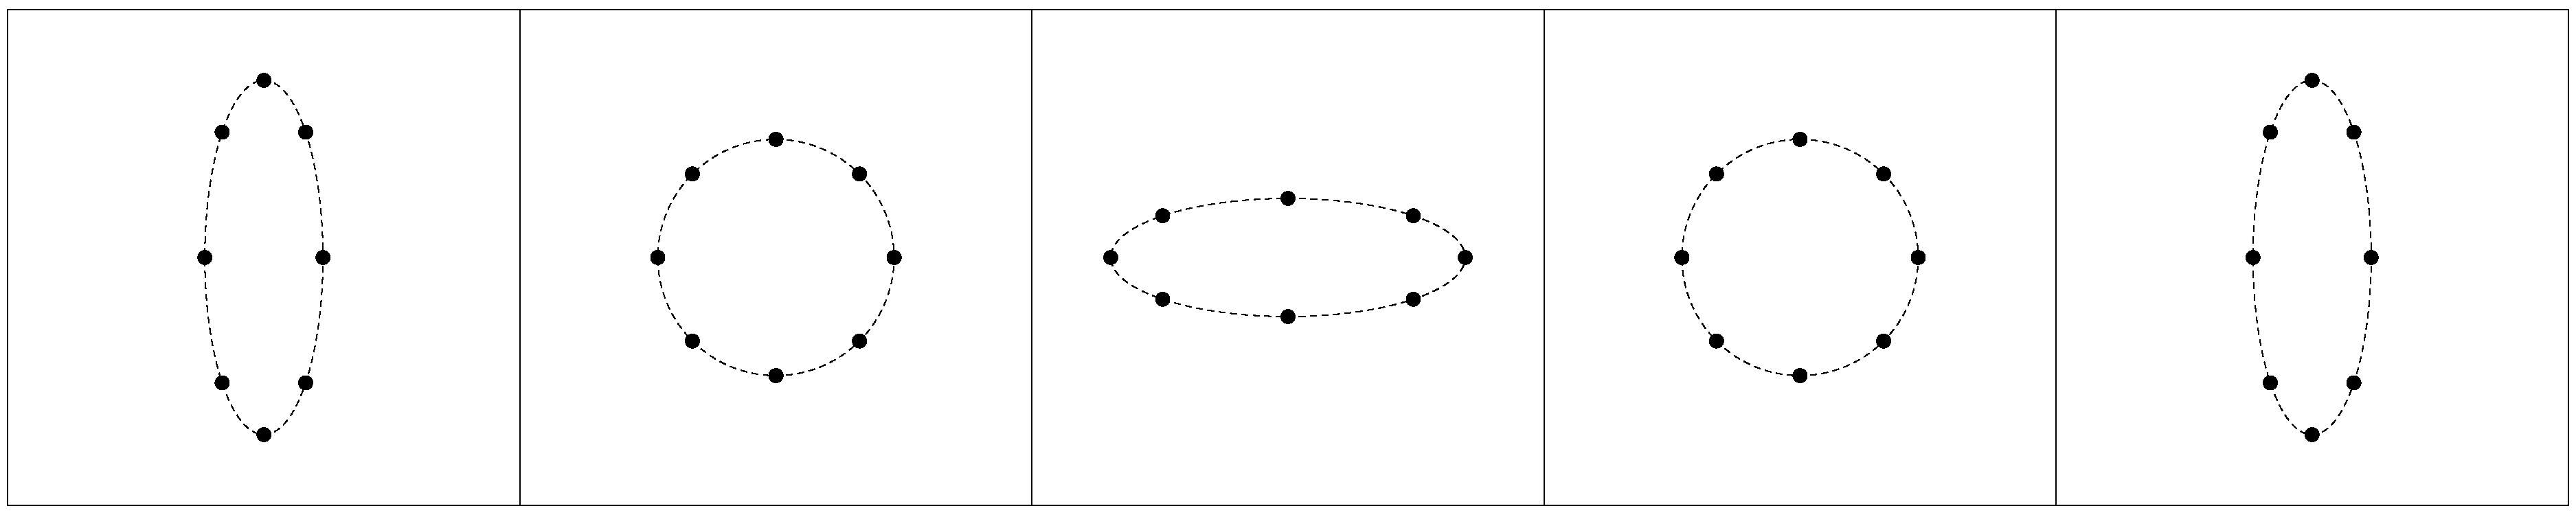
\includegraphics[width=\textwidth]{effect_gw.pdf}
\caption[Effect of GW on ring of test masses]{This image is taken from \cite{bachelor}. It shows the effect of a \gls{gw} passing orthogonaly through a ring of test masses.}\label{fig:gw_test_masses}
\end{figure}
\eqref{def:gw_wave_equation} shows, that \gls{gw} exist and can travel through space. It does however not specify how these waves are produced. To do so, the energy-momentum-tensor cannot be set to $0$. Instead the full equation \eqref{def:gw_equation} needs to be solved. The solution is known to be
\begin{equation}
\bar{h}\lr{t, \vec{x}}=\frac{4 G}{c^4}\int\Diff{3}x'\ \frac{T_\mn\lr{t-\frac{\norm{\vec{x}-\vec{x}'}}{c},\vec{x}'}}{\norm{\vec{x}-\vec{x}'}}.
\end{equation}
For simplification it is assumed, that the observer is far from the source when compared to the size of the support of $T_\mn$, such that $\norm{\vec{x}-\vec{x}'}\approx r\coloneqq\norm{\vec{x}}$. Therefore we need to solve
\begin{equation}
\bar{h}\lr{t, \vec{x}}=\frac{4 G}{c^4}\frac{1}{r}\int\Diff{3}x'\ T_\mn\lr{t-\frac{r}{c},\vec{x}'}.
\end{equation}
This equation can be solved to yield
\begin{equation}
h_{ab}^\text{\gls{tt}}\lr{t,\vec{x}}=\frac{2 G}{c^4}\frac{1}{r}\ddot{I}_{ab}^\text{\gls{tt}}\lr{t-r/c},
\end{equation}
where $\ddot{I}_{ab}^\text{\gls{tt}}$ is the transverse-traceless-projection of the second time derivative of the second mass moment
\begin{equation}\label{def:quad_st_1}
\ddot{I}^{ab}=c^2\partial_0^2 \int\Diff{3}x'\ x'^a x'^b T^{00} = 2\int\Diff{3}x'\ T^{ab}.
\end{equation}
As the quadrupole moment is simply the traceless second mass moment and we project it to its traceless part anyways, \eqref{def:quad_st_1} can be rewritten as
\begin{equation}\label{def:h_quadrupole}
\boxed{h^{\gls{tt}}_{ab}\lr{t,\vec{x}} = \frac{2 G}{c^4}\frac{1}{r}\ddot{Q}^{\gls{tt}}_{ab}\lr{t-r/c},}
\end{equation}
with $Q_{ab}\coloneqq I_{ab} - \frac{1}{3}\delta_{ab}I^c_c$. This is the famous quadrupole formula. (chapter 5.2 in \cite{bachelor})\medskip\\

\noindent To calculate the \gls{gw} a binary system emtis, $I_{ab}$ or $Q_{ab}$ needs to be specified. Furthermore the transverse-traceless-projection needs to be calculated. The projection turns out to be ((3.64) in \cite{gwv1})
\begin{equation}
\ddot{I}_{ab}^\text{\gls{tt}}=
\begin{pmatrix}
\lr{\ddot{I}_{11}-\ddot{I}_{22}}/2 & \ddot{I}_{12}                     & 0\\
\ddot{I}_{21}                      & -\lr{\ddot{I}_{11}-\ddot{I}_{22}}/2 & 0\\
0                                  & 0                                 & 0
\end{pmatrix}_{ab}.
\end{equation}
Therefore the waveforms are given by
\begin{align}
h_+ & = \frac{1}{r}\frac{G}{c^4}\lr{\ddot{I}_{11}-\ddot{I}_{22}}\\
h_\times & = \frac{2}{r}\frac{G}{c^4}\ddot{I}_{12}.
\end{align}
The approximations, that led to \eqref{def:einstein_linear}, restrict the validity of the results above to the case, where there are only slight perturbations to the flat space-time. Therefore the motion of a binary system can be well approximated by classical mechanics. Therefore assume a system of two point-particles with masses $m_1$, $m_2$ that orbit each other in circular motion. In Newtonian mechanics, this problem reduces to an effective one body problem with the reduced mass $\mu=\frac{m_1m_2}{m_1+m_2}$. The motion in these relative coordinates is given by
\begin{equation}\label{def:binary_motion}
\vec{r}\lr{t} = R\cdot
\begin{pmatrix}
	-\sin\lr{\omega_s t}\\
	\cos\lr{\omega_s t}\\
	0
\end{pmatrix},
\end{equation}
where $R$ is the orbital separation of the two point masses and $\omega_s$ the orbital frequency. From this one gets
\begin{equation}\label{def:binary_system_second_mass_moment}
\left[ I^{ab}\right] = \mu R^2\begin{pmatrix}
		\sin^2\lr{\omega_s t} & -\frac{1}{2}\sin\lr{2\omega_s t} & 0\\
		-\frac{1}{2}\sin\lr{2\omega_s t} & \cos^2\lr{\omega_s t} & 0\\
		0 & 0 & 0
	\end{pmatrix}
\end{equation}
and subsequently
\begin{equation}\label{def:binary_system_second_mass_moment_time_derivative}
\left[ \ddot{I}^{ab}\right] = 2 \mu R^2\omega_s^2
	\begin{pmatrix}
		\cos\lr{2\omega_s t} & \sin\lr{2\omega_s t} & 0\\
		\sin\lr{2\omega_s t} & -\cos\lr{2\omega_s t} & 0\\
		0 & 0 & 0
	\end{pmatrix}.
\end{equation}
Therefore the amplitudes are given by
\begin{align}\label{def:gw_source_frame}
h_+ &= \frac{4}{r}\frac{G}{c^4}\mu R^2 \omega_s^2\cos\lr{2\omega_s t}\nonumber\\
h_\times &= \frac{4}{r}\frac{G}{c^4}\mu R^2 \omega_s^2\sin\lr{2\omega_s t}.
\end{align}
Interestingly the frequency of the \gls{gw} is twice the frequency of the orbital period.\\
The equations \eqref{def:gw_source_frame} are written in the source frame, i.e. they are the \gls{gw}-polarizations emitted in the z-direction, where the z-axis is the one orthogonal to the orbital plane and at the center of gravity. When measuring these waves however, we are not assured, that the system emits face-on to our detectors. Therefore we need to change coordinates, to get the emission in a general direction $\hat{n}$. To do so, one simply has to transform the second mass moment into the new frame. These calculations can be found on p.111 in \cite{gwv1} and finally yield
\begin{align}\label{def:gw_travel_direction}
h_+ &= \frac{4}{r}\frac{G}{c^4}\mu R^2 \omega_s^2\lr{\frac{1+\cos^2\lr{\iota}}{2}}\cos\lr{2\omega_s t+2\Phi}\nonumber\\
h_\times &= \frac{4}{r}\frac{G}{c^4}\mu R^2 \omega_s^2\cos\lr{\iota}\sin\lr{2\omega_s t+2\Phi},
\end{align}
where $\iota$ is the inclination and $\Phi$ is the phase of the wave at $t=0$.\medskip\\
To be measured, these waves need to hit a detector. The most common and currently only operational \gls{gw}-detectors are advanced Michelson-interferometers, with an angle of $\pi/2$ between the two arms. If the \gls{gw} hits such a detector, it will cause a deviation $\delta l$ in arm lengths given by the detector response functions
%\delta l = F_+\lr{\theta, \varphi} h_+ + F_\times\lr{\theta, \varphi} h_\times,
\begin{equation}\label{def:detector_response}
\delta l = F_+\lr{\theta, \varphi}\lr{\cos\lr{2\psi}h_+ - \sin\lr{2\psi} h_\times} + F_\times\lr{\theta, \varphi}\lr{\sin\lr{2\psi}h_+ + \cos\lr{2\psi} h_\times},
\end{equation}
with $h_+$ and $h_\times$ as given in \eqref{def:gw_travel_direction} and
\begin{align}
F_+\lr{\theta, \varphi} &\coloneqq \frac{1}{2}\lr{1+\cos^2\lr{\theta}}\cos\lr{2\varphi}\nonumber\\
F_\times\lr{\theta, \varphi} &\coloneqq\cos\lr{\theta}\sin\lr{2\varphi}.
\end{align}
The angle $\theta$ is the angle between the propagation direction of the \gls{gw} to the (outwards facing) normal of the detector. $\varphi$ is the angle between one arm of the detector\footnote{If the arms were labeled with $x$ and $y$ in such a way, that they form a right handed coordinate system with the outwards facing normal vector, the arm the angle $\varphi$ is taken to is the one labeled $x$.} to the projection of the propagation direction of the \gls{gw} into the detector-plane. Therefore the angles $\theta$ and $\varphi$, or rather their projection onto a global coordinate system, are the declination and right ascension respectively. The angle $\psi$ is known as the polarization angle and is not detectable for a single detector. This is due to the reason, that rotating the wave around its propagation axis has the same effect.\medskip\\
All the calculations above disregarded the energy carried away by the \gls{gw}. To include it, one needs to calculate the luminosity of a \gls{gw}-source, which in turn requires the computation of an effective energy-momentum tensor of the \gls{gw} itself.\\
To get this energy-momentum-tensor, second order corrections in $h$ of $R_\mn$ need to be computed and averaged over time. As a result one gets \textcolor{red}{[Citation]}
\begin{equation}
t_\mn = \frac{c^4}{32\pi G}\langle\partial_\mu h^{\sigma\alpha}\partial_\nu h_{\sigma\alpha}\rangle.
\end{equation}
The luminosity is the energy flux at spatial infinity and thus given by
\begin{equation}
L_\text{\gls{gw}} = \lim_{r\to\infty}\int_{S^2\lr{r}}\diff\vec{n}\ \vec{S},
\end{equation}
where $S^i=-c\cdot t^{0i}$ and $S^2\lr{r}$ denotes the spherical shell of radius $r$. When solving this integral and using \eqref{def:h_quadrupole} one gets
\begin{equation}\label{def:luminosity_quadrupole}
\boxed{L_\text{\gls{gw}}=\frac{G}{5c^5}\langle\dddot{Q}^{ab}\dddot{Q}_{ab}\rangle.}
\end{equation}
This equation can now be applied to the binary system specified by \eqref{def:binary_system_second_mass_moment}. To simplify notation and to give measurable parameters, denote, that the dynamics of the system under consideration are governed by Newtonian physics and thus Kepler's laws apply. Especially Kepler's third law
\begin{equation}\label{def:kepler_third_law}
\omega_s^2=\frac{G M}{R^3}
\end{equation}
will be of use, where $M=m_1+m_2$ is the total mass of the system. Using \eqref{def:kepler_third_law} to eliminate $R$ in \eqref{def:binary_system_second_mass_moment} and inserting this equation into \eqref{def:luminosity_quadrupole} yields
\begin{equation}\label{def:luminoisity_binary_system}
L_\text{\gls{gw}}=\frac{32}{5}\frac{c^5}{G}\lr{\frac{G\omega_s M_c}{c^3}}^{10/3},
\end{equation}
where
\begin{equation}
M_c\coloneqq \mu^{3/5}M^{2/5}=\frac{\lr{m_1 m_2}^{3/5}}{\lr{m_1 + m_2}^{1/5}}.
\end{equation}
$M_c$ is called the chirp mass and is the only mass-combination a \gls{gw} depends on in linearized theory.\medskip\\
According to \eqref{def:luminoisity_binary_system} a binary system looses energy when emitting \gls{gw}. The energy that is carried away, is taken from the orbital energy $E_\text{orbit}$ of the binary system. Therefore, disregarding any other effects\footnote{These effects could for instance be tidal deformation, mass acquisition or other sources of gravity in the proximity of the binary system.}, that might cause $E_\text{orbit}$ to vary,
\begin{equation}
-\frac{d E_\text{orbit}}{dt}=-\frac{1}{2}\frac{G m_1 m_2 \dot{R}}{R^2}\mbe L_\text{\gls{gw}}.
\end{equation}
One can again utilize \eqref{def:kepler_third_law} to eliminate $R$ and $\dot{R}$ in favor of $\omega_s$ and $\dot{\omega}_s$. Furthermore, $\omega_s = \pi f_\text{\gls{gw}}$, and thus
\begin{equation}\label{def:frequency_evolution_differential}
\dot{f}_\text{\gls{gw}}=\frac{96}{5}\pi^{8/3}\lr{\frac{G M_c}{c^3}}^{5/3}f_\text{\gls{gw}}^{11/3}.
\end{equation}
This equation describes a runaway process, as for a positive value $f_\text{\gls{gw}}$ the change in frequency is positive, leading to a larger value of $f_\text{\gls{gw}}$ and so on. This in turn by \eqref{def:kepler_third_law} means, that the two masses will come closer and closer together until they touch. This point, where the waveform shuts of gives a specific point in time, which will be denoted by $t_\text{coal}$. With this, one can define the time till coalescence $\tau=t_\text{coal}-t$ and solve the differential equation \eqref{def:frequency_evolution_differential}. \textcolor{red}{[Cite p.170 \cite{gwv1}]}
\begin{equation}\label{def:frequency evolution}
f_\text{\gls{gw}}\lr{\tau} = \frac{1}{\pi}\lr{\frac{5}{256}\frac{1}{\tau}}^{3/8}\lr{\frac{G M_c}{c^3}}^{-5/8}
\end{equation}
Now that the frequency evolution of a \gls{gw} is known, the amplitudes $h_+$ and $h_\times$ can also be modeled. To do so revisit the initial assumption \eqref{def:binary_motion}. In this equation $R$ will now be time dependent and $\omega_s t$ will be replaced by $\Phi\lr{t}$, with
\begin{equation}\label{def:phase_equation}
\Phi\lr{t} = 2\pi \int_{t_0}^t\diff t'\ f_\text{\gls{gw}}\lr{t'}.
\end{equation}
In principle all time derivatives in \eqref{def:binary_system_second_mass_moment_time_derivative} would need to be redone, taking into account the time dependence of $\omega_s$ and $R$. However, the approximations that have lead to these waveforms are quite strong. $\dot{\omega}_s$ and $\dot{R}$ will only have non-negligible contributions, when frequencies are pretty high and the orbital separation $R$ is small. In these regimes the linear approximation \eqref{def:linear_approximation} will be invalid. Therefore we can neglect the contributions of $\dot{\omega}_s$ and $\dot{R}$ and still get a qualitative look into the dynamics of the system. Hence replace $\omega_s$ in the prefactor of \eqref{def:gw_travel_direction} by $\pi f_\text{\gls{gw}}\lr{t}$, $2\omega_s t + 2 \Phi$ by $\Phi\lr{t}$ and $R$ by \eqref{def:kepler_third_law}.\\
With \eqref{def:frequency evolution} equation \eqref{def:phase_equation} can be solved to yield
\begin{equation}
\Phi\lr{\tau}=-2\lr{\frac{5 G M_c}{c^3}}^{-5/8}\tau^{5/8}+\Phi_0,
\end{equation}
where $\Phi_0$ is the phase at $\tau=0$, i.e. at coalescence. Therefore this value is called the coalescence phase. Combining these results, one gets the time dependent waveforms
\begin{align}\label{def:linear_waveforms_time_evolution}
h_+\lr{t} & = \frac{1}{r}\lr{\frac{G M_c}{c^2}}^{5/4}\lr{\frac{5}{c\tau}}^{1/4}\lr{\frac{1+\cos^2\lr{\iota}}{2}}\cos\lr{\Phi\lr{\tau}}\nonumber\\
h_\times\lr{t} & = \frac{1}{r}\lr{\frac{G M_c}{c^2}}^{5/4}\lr{\frac{5}{c\tau}}^{1/4}\cos\lr{\iota}\cos\lr{\Phi\lr{\tau}}.
\end{align}
Combining \eqref{def:detector_response} and \eqref{def:linear_waveforms_time_evolution} shows, that in linearized theory the output of a detector depends on 8 parameters. These are the luminosity distance $r$, the cirp-mass $M_c$, the coalescence time $t_\text{coal}$, the coalescence phase $\Phi_0$, the inclination $\iota$, the declination $\theta$, the right ascension $\varphi$ and the polarization angle $\psi$. The first four parameters are source intrinsic parameters, where $M_c$ is a combination of the component masses $m_1$ and $m_2$. In that sense the parameter space can be extended to be 9-dimensional.\\
\autoref{fig:linear_waveform} shows an example of the time evolution of a waveform \eqref{def:linear_waveforms_time_evolution}.\medskip\\
\begin{figure}
\centering
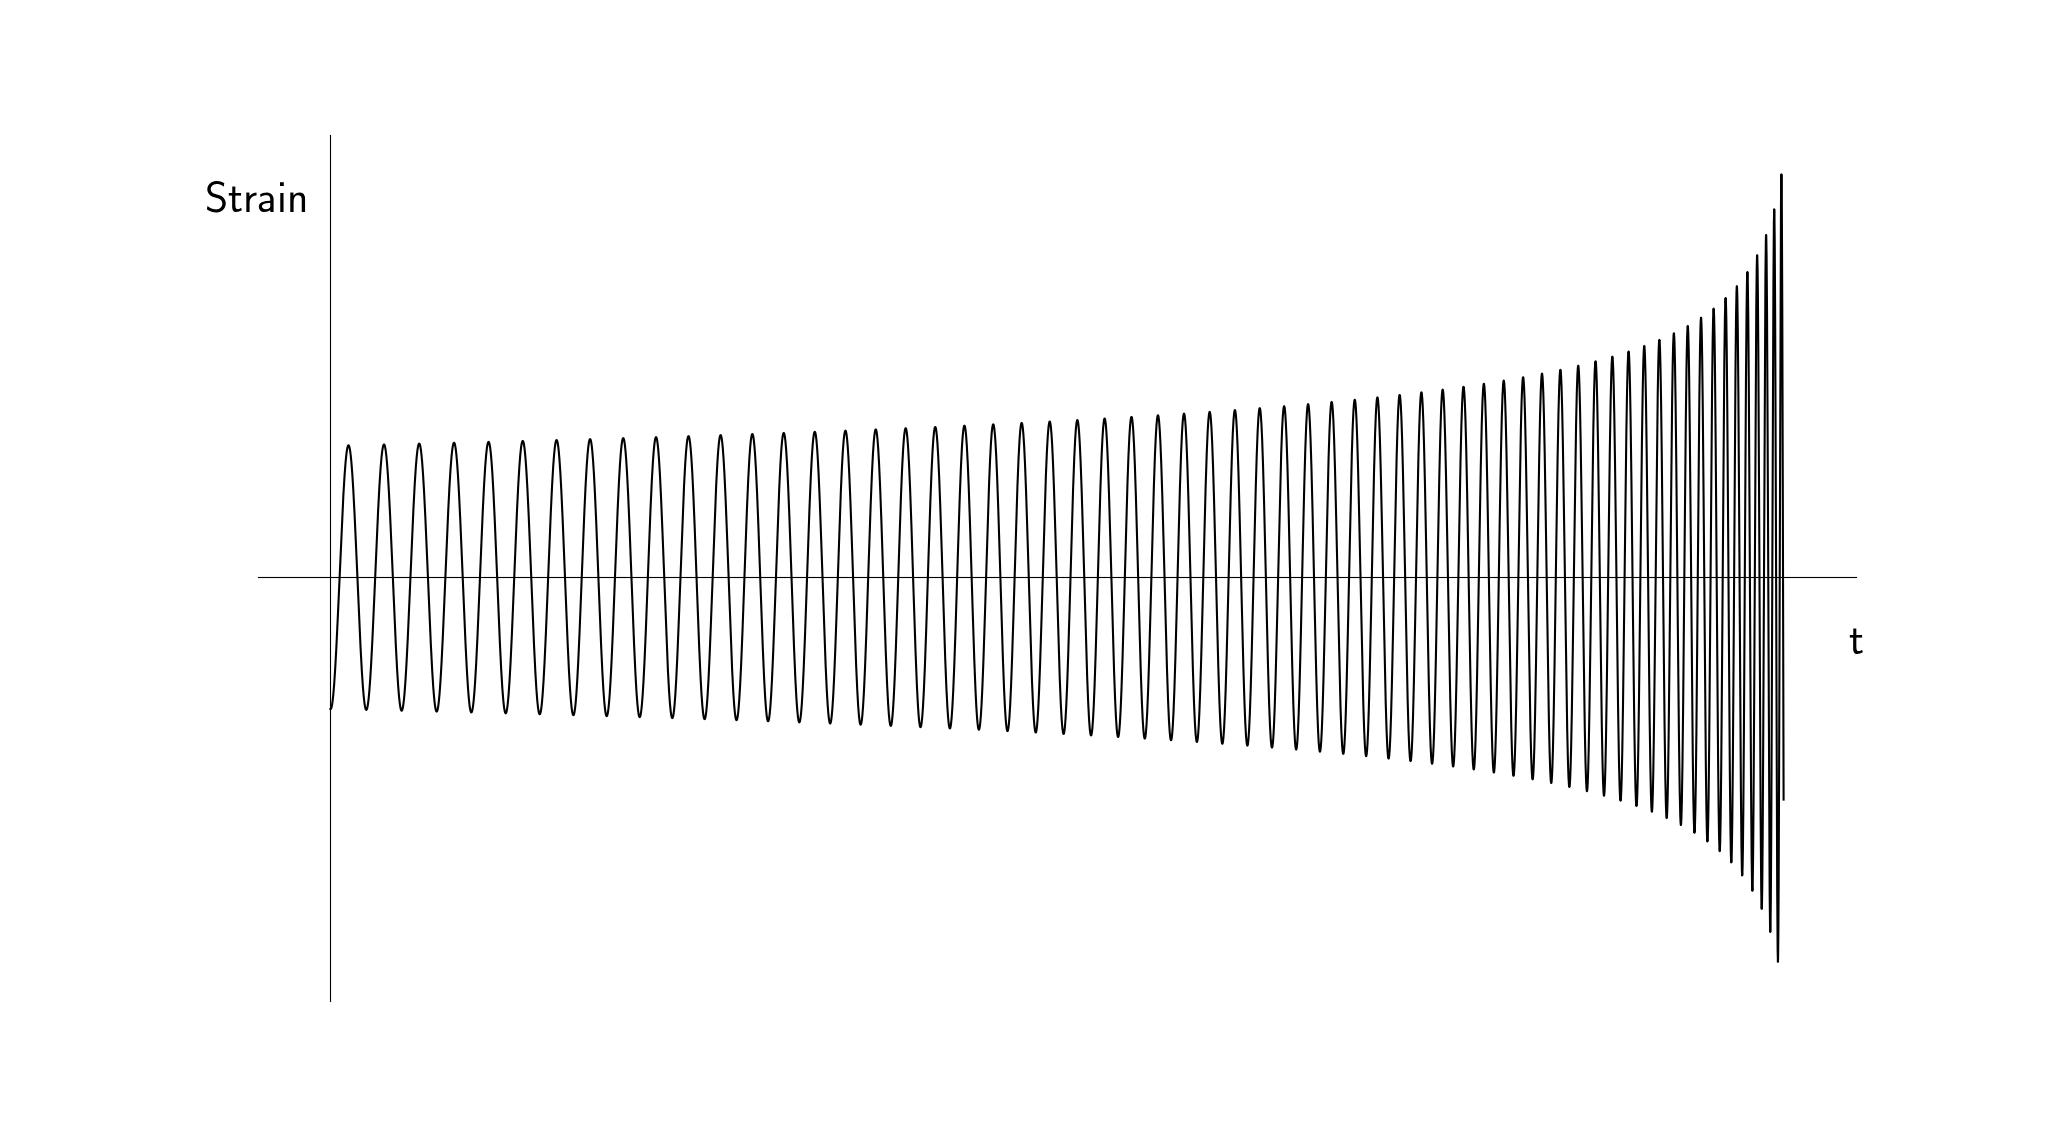
\includegraphics[width=\textwidth]{linear_waveform.png}
\caption[Example time-evolution of a linear waveform]{This figure is heavily based on Figure 4.1 in \cite{gwv1}. Shown is an example of a waveform as it could be observed by a detector if the linear waveforms describe the source accuratly. Note the frequency and amplitude evolution. Both rise simultaniously. This behavior is called ''chirping''.}\label{fig:linear_waveform}
\end{figure}
Until now, the approximations made were quite strict. One of the major ones is the approximation of the two bodies of mass $m_1$ and $m_2$ as point particles. As such they have no intrinsic spin. Dropping this restriction shows, that also angular momentum is radiated away. Also each \textcolor{red}{Spin seems to be difficult. If it doesn't fit time wise, consider just pointing out, that there are in theory 6 more parameters coming from the individual spins, but as we only look at non-spinning systems anyways, we will not go into further detail and the effects here. Otherwise maybe look at Stephans Bachelor thesis to get a little grasp on spins and their effects? However I'm not comfortable writing, that spins only come into effect in PN-theory. Maybe I can find a mass momentum $I^{ab}$ for a binary system of two spinning masses and just say, that this can be plugged into the according equations?}\\
\textcolor{red}{Include backreaction in first order as 4.1.1 \cite{gwv1} does, until equation (4.32). Mention that elliptic effects can be mostly disregarded, cite \cite{gwv1}. Go over into PN territory and mention what changes.}

\subsection{Matched filtering}
\textcolor{blue}{Explain what matched filtering is, why it works and how it is applied currently.}